% Lecture Template for ME3023 -  Measurements in Mechanical Systems - Tennessee Technological University
% Spring 2020 - Summer 2020 - Fall 2020 - Spring 2021 - Summer 2021 - Fall 2023
% Tristan Hill, May 07, 2020 - June 12, 2020 - July 08, 2020 - Novemeber 02, 2020 - March 28, 2021 - May 25, 2021 - August 21, 2022 - September 02, 2023 - September 09, 2023 - March 24, 2024

% Fall 2023 - condensing and streamlining lectures by combining topics into a single PDF under the module name
%			  this will simplify file and link management as well as make lectures easier to use in class
%			- added image/ to clean directory and reduce redundancy, specific to module for now  

% Module Name: - Data Acquisition
% Topic 1 -
% Topic 2 -
% Topic 3 -


\documentclass[fleqn]{beamer} % for presentation (has nav buttons at bottom)

%\usepackage{/home/tntech.edu/thill/courses/measurements/lectures/measurements_lectures}
%\usepackage{/home/thill/courses/measurements/lectures/measurements_lectures}
\usepackage{/mnt/c/Users/thill/Documents/courses/measurements/lectures/measurements_lectures}

\author{ME3023 - Measurements in Mechanical Systems} 

\newcommand{\MNUM}{8\hspace{2mm}} % module number 
\newcommand{\moduletitle}{Data Acquisition}

\newcommand{\sectionItitle}{Analog to Digitial Conversion}
\newcommand{\sectionIItitle}{}
\newcommand{\sectionIIItitle}{}

\newcommand{\sectionIsubsectionItitle}{DAQ and Computer Storage}
\newcommand{\sectionIsubsectionIItitle}{Number Types}
\newcommand{\sectionIsubsectionIIItitle}{Analog to Digital Conversion and DAQ}
\newcommand{\sectionIsubsectionIVtitle}{Activity: ADC Resolution Calculation}

\newcommand{\sectionIIsubsectionItitle}{}
\newcommand{\sectionIIsubsectionIItitle}{}
\newcommand{\sectionIIsubsectionIIItitle}{}
\newcommand{\sectionIIsubsectionIVtitle}{}

\newcommand{\sectionIIIsubsectionItitle}{}
\newcommand{\sectionIIIsubsectionIItitle}{}
\newcommand{\sectionIIIsubsectionIIItitle}{}
\newcommand{\sectionIIIsubsectionIVtitle}{}

 \newcommand{\btVFill}{\vskip0pt plus 1filll}

% custom box
\newsavebox{\mybox}

\title{Lecture Module - \moduletitle}

\date{Mechanical Engineering\vspc Tennessee Technological University}

\begin{document}

	\lstset{language=MATLAB,basicstyle=\ttfamily\small,showstringspaces=false}

	\frame{\titlepage \center\begin{framed}\Large \textbf{Module \MNUM - \moduletitle}\end{framed} \vspace{5mm}}

	% Module Outline
	\begin{frame} 
		\large \textbf{Module \MNUM - \moduletitle} \vspace{3mm}\\

		\begin{itemize}
			\item Topic 1 - \hyperlink{sectionI}{\sectionItitle} \vspc % section I
			\item Topic 2 - \hyperlink{sectionII}{\sectionIItitle} \vspc % section II
			\item Topic 3 - \hyperlink{sectionIII}{\sectionIIItitle} \vspc % section III
		\end{itemize}

	\end{frame}

	% section I
	\section{\sectionItitle}\label{sectionI}

		% section I Outline
		\begin{frame} 
			\large \textbf{Topic 1 - \sectionItitle} \vspace{3mm}\\

			\begin{itemize}
				\item \hyperlink{sectionIsubsectionI}{\sectionIsubsectionItitle} \vspc %  section I subsection I
				\item \hyperlink{sectionIsubsectionII}{\sectionIsubsectionIItitle} \vspc % section I subsection II
				\item \hyperlink{sectionIsubsectionIII}{\sectionIsubsectionIIItitle} \vspc % section I subsection III
				\item \hyperlink{sectionIsubsectionIV}{\sectionIsubsectionIVtitle} \vspc % section I subsection IV
			\end{itemize}
		\end{frame}
		
		% section I subsection I 
		\subsection{\sectionIsubsectionItitle}\label{sectionIsubsectionI}

			\begin{frame}
				\frametitle{\sectionIsubsectionItitle}

				A data acquisition system is the portion of a measurement system that quantifies and stores data. - {\tiny Theory and Design of Mechanical Measurements}

				\begin{multicols}{2}
				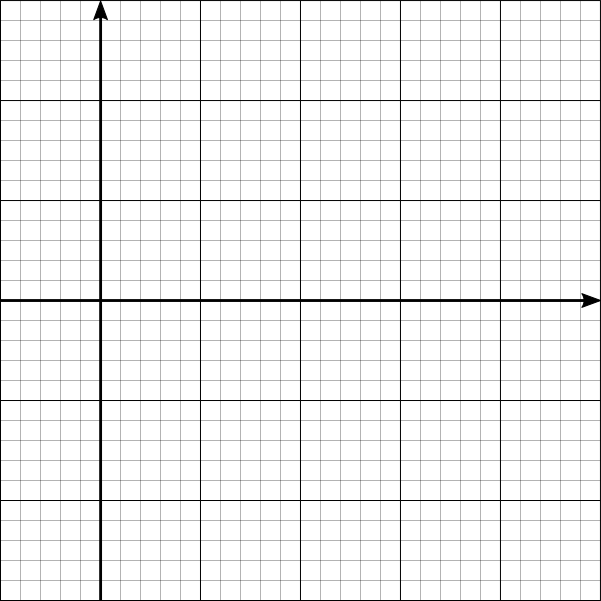
\includegraphics[scale=.30]{images/cartesian_6x6_B.png} 
				

				\end{multicols}
				\btVFill
				\tiny{Image: T.Hill}
	
			\end{frame}

			\begin{frame}
				\frametitle{\sectionIsubsectionItitle}

		
	

		

			\end{frame}

		% section I subsection II
		\subsection{\sectionIsubsectionIItitle}\label{sectionIsubsectionII}

			\begin{frame}
				\frametitle{\sectionIsubsectionIItitle}\small
				\bigskip

				\begin{itemize}

					\item Integers 

						\begin{itemize}
							\item Binary
							\item Decimal
							\item Hexadecimal
						\end{itemize}

					\item Fixed Point 		

					\item Floating Point 



				\end{itemize}

				\btVFill
				

			\end{frame}

			\begin{frame}
				\frametitle{\sectionIsubsectionIItitle}\small
				\bigskip

				\begin{multicols}{2}
				\begin{tabular}{|r|r|r|} \hline
					Binary 	& Decimal 	& Hexadecimal \\ \hline
					0		& 0			& 0 		\\ \hline	
					1		& 1			& 1 		\\ \hline
					10		& 2			& 2 		\\ \hline
					11		& 3			& 3 		\\ \hline
					100		& 4			& 4 		\\ \hline
							& 5			& 5 		\\ \hline
							& 6			& 6 		\\ \hline
						    & 7			& 7 		\\ \hline
							& 8			& 8 		\\ \hline
							& 9			& 9 		\\ \hline
							& 10		& A 		\\ \hline
							& 11		& B 		\\ \hline
				\end{tabular}

				\begin{tabular}{|r|r|r|} \hline
					Binary 	& Decimal 	& Hexadecimal \\ \hline
							& 12		& C 		\\ \hline	
							& 13		& D 		\\ \hline
							& 14		& E 		\\ \hline
							& 15		& F 		\\ \hline
							& 16		&  		\\ \hline
							& 17		&  		\\ \hline
							& 18		&  		\\ \hline
							& 19		&  		\\ \hline
							& 20		&  		\\ \hline
							& 21		&  		\\ \hline
							& 22	    &  		\\ \hline
							& 23	    &  		\\ \hline
				\end{tabular}
				\end{multicols}

				\btVFill
				\tiny{some reference}		

			\end{frame}

			\begin{frame}
				\frametitle{\sectionIsubsectionIItitle} \small
				\bigskip

				\begin{multicols}{2}
				\begin{tabular}{|r|r|r|} \hline
					Binary 	& Decimal 	& Hex. \\ \hline
					0		& 0			& 0 		\\ \hline	
					1		& 1			& 1 		\\ \hline
					10		& 2			& 2 		\\ \hline
					11		& 3			& 3 		\\ \hline
					100		& 4			& 4 		\\ \hline
					& 			&  		\\ \hline
					& 			&  		\\ \hline
					& 			&  		\\ \hline
					& 			&  		\\ \hline
					& 			&  		\\ \hline
					& 		&  		\\ \hline
					& 		&  		\\ \hline
				\end{tabular}

				\begin{tabular}{|r|r|r|} \hline
					Binary\hspace{18mm} 	& Decimal 	& Hex. \\ \hline
					0		& 0			& 0 		\\ \hline	
					1		& 1			& 1 		\\ \hline
					10		& 2			& 2 		\\ \hline
					11		& 3			& 3 		\\ \hline
					100		& 4			& 4 		\\ \hline
					& 			&  		\\ \hline
					& 			&  		\\ \hline
					& 			&  		\\ \hline
					& 			&  		\\ \hline
					& 			&  		\\ \hline
					& 		&  		\\ \hline
					& 		&  		\\ \hline
				\end{tabular}
				\end{multicols}

				\btVFill
				\tiny{some reference}	


			\end{frame}


			\begin{frame}

				\frametitle{\sectionIsubsectionIItitle} \small
				\bigskip




			  	Standard storage of a floating point value in memory\\	

			  	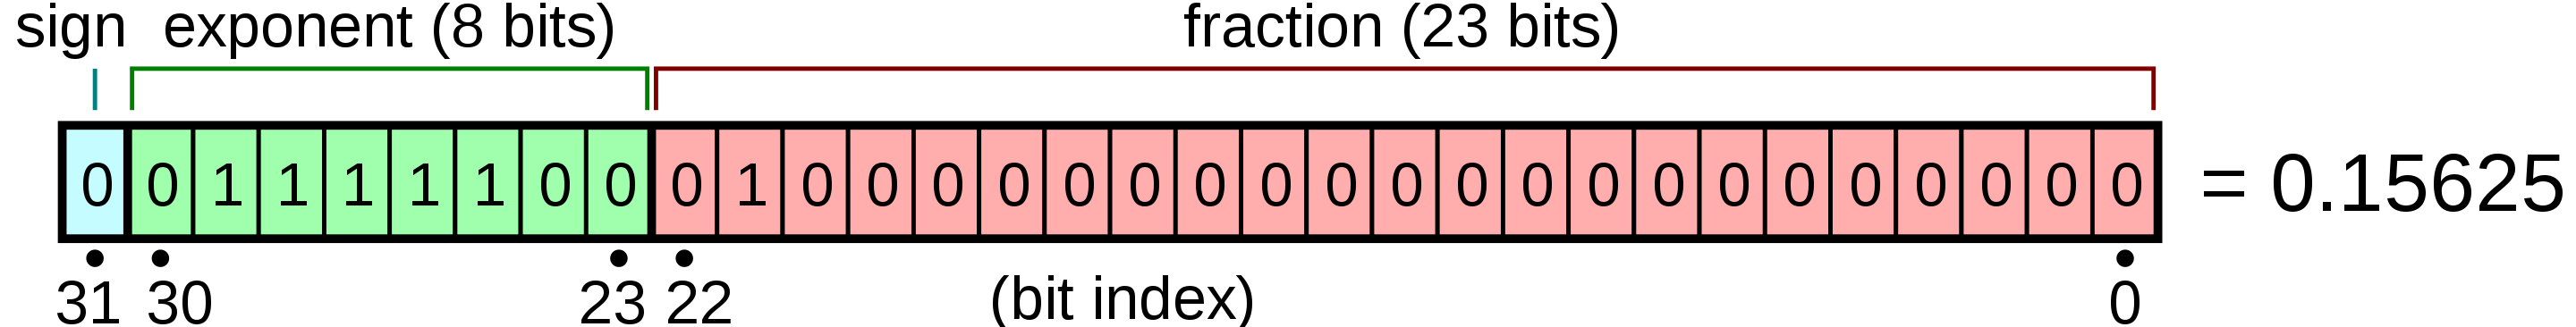
\includegraphics[scale=.10]{images/ieee754_bits.png}	
			  	\btVFill
				
				{\tiny \href{https://en.wikipedia.org/wiki/IEEE_754}{Wikipedia: IEEE Float} \href{https://en.wikipedia.org/wiki/Fixed-point_arithmetic}{Wikipedia: Fixed Point} }

			\end{frame}

			\begin{frame}
			\bigskip 


			
			\btVFill
			\tiny{Text: Theory and Design for Mechanical Measurements}	
			\end{frame}





		% section I subsection III
		\subsection{\sectionIsubsectionIIItitle}\label{sectionIsubsectionIII}
			\begin{frame} 
				\frametitle{\sectionIsubsectionIIItitle}

				\bigskip

					
				\btVFill
				\tiny{Text: Theory and Design for Mechanical Measurements}	

			\end{frame}	

			\begin{frame} 
				\frametitle{\sectionIsubsectionIIItitle}

				
			\end{frame}	

		% section I subsection IV
		\subsection{\sectionIsubsectionIVtitle}\label{sectionIsubsectionIV}	

			\begin{frame}
				\frametitle{\sectionIsubsectionIVtitle}
				\bigskip


				\btVFill
				\tiny{Text: Theory and Design for Mechanical Measurements}

			\end{frame}

			\begin{frame}
				\frametitle{\sectionIsubsectionIVtitle}

				\bigskip


				\btVFill
				\tiny{: Theory and Design for Mechanical Measurements}
										
			\end{frame}

	
	% Section II
	\section{\sectionIItitle}\label{sectionII}

		% section II Outline
		\begin{frame}
			\large \textbf{Topic 2 - \sectionIItitle} \vspace{3mm}\\

			\begin{itemize}
				\item \hyperlink{sectionIIsubsectionI}{\sectionIIsubsectionItitle} \vspc %  section II subsection I
				\item \hyperlink{sectionIIsubsectionII}{\sectionIIsubsectionIItitle} \vspc % section II subsection II
				\item \hyperlink{sectionIIsubsectionIII}{\sectionIIsubsectionIIItitle} \vspc % section II subsection III
				\item \hyperlink{sectionIIsubsectionIV}{\sectionIIsubsectionIVtitle} \vspc % section II subsection IV
			\end{itemize}

		\end{frame}

		% section II subsection I
		\subsection{\sectionIIsubsectionItitle}\label{sectionIIsubsectionI}

			\begin{frame}[label=sectionIIsubsectionI]
				\frametitle{\sectionIIsubsectionItitle}

				\btVFill
				\tiny{Text: Theory and Design for Mechanical Measurements}
		
			\end{frame}

		    \begin{frame}[label=sectionIIsubsectionI]
				\frametitle{\sectionIIsubsectionItitle}


			\end{frame}	

		% section II subsection II
		\subsection{\sectionIIsubsectionIItitle}\label{sectionIIsubsectionII}

			\begin{frame}
				\frametitle{\sectionIIsubsectionIItitle}



			\end{frame}

		% section II subsection III
		\subsection{\sectionIIsubsectionIIItitle}\label{sectionIIsubsectionIII}

			\begin{frame}
				\frametitle{\sectionIIsubsectionIIItitle}


				\btVFill
				\tiny{ : Theory and Design for Mechanical Measurements}

			\end{frame}

			\begin{frame}
				\frametitle{\sectionIIsubsectionIIItitle}

				\bigskip


				\btVFill
				\tiny{: Theory and Design for Mechanical Measurements}	
			
			\end{frame}

			\begin{frame}
			\frametitle{\sectionIIsubsectionIIItitle}




				\btVFill
				\tiny{ : Theory and Design for Mechanical Measurements}	

			\end{frame}

		% section II subsection IV 
		\subsection{\sectionIIsubsectionIVtitle}\label{sectionIIsubsectionIV}

			\begin{frame}
				\frametitle{\sectionIIsubsectionIVtitle}


			\end{frame}

			\begin{frame}
				\frametitle{\sectionIIsubsectionIVtitle}


			\end{frame}
		
	% Section III
	\section{\sectionIIItitle}\label{sectionIII}

		% section III Outline
		\begin{frame}
			\large \textbf{Topic 3 - \sectionIIItitle} \vspace{3mm}\\

			\begin{itemize}
				\item \hyperlink{sectionIIIsubsectionI}{\sectionIIIsubsectionItitle} \vspc %  section III subsection I
				\item \hyperlink{sectionIIIsubsectionII}{\sectionIIIsubsectionIItitle} \vspc % section III subsection II
				\item \hyperlink{sectionIIIsubsectionIII}{\sectionIIIsubsectionIIItitle} \vspc % section III subsection III
				\item \hyperlink{sectionIIIsubsectionIV}{\sectionIIIsubsectionIVtitle} \vspc % section III subsection IV
			\end{itemize}

		\end{frame}

		% section III subsection I
		\subsection{\sectionIIIsubsectionItitle}\label{sectionIIIsubsectionI}

			\begin{frame}
				\frametitle{\sectionIIIsubsectionItitle}

			
				
			\end{frame}

			\begin{frame}
				\frametitle{\sectionIIIsubsectionItitle}
		
			\end{frame}

		% section III subsection II
		\subsection{\sectionIIIsubsectionIItitle}\label{sectionIIIsubsectionII}	

			\begin{frame}
				\frametitle{\sectionIIIsubsectionIItitle}

	

			\end{frame}

		% section III subsection III
		\subsection{\sectionIIIsubsectionIItitle}\label{sectionIIIsubsectionIII}

			\begin{frame}
				\frametitle{\sectionIIIsubsectionIIItitle}

		

			\end{frame}

			\begin{frame}
				\frametitle{\sectionIIIsubsectionIIItitle}



			\end{frame}

		% section III subsection IV
		\subsection{\sectionIIIsubsectionIVtitle}\label{sectionIIIsubsectionIV}	

			\begin{frame}
				\frametitle{\sectionIIIsubsectionIVtitle}

			


			\end{frame}

			\begin{frame}
				\frametitle{\sectionIIIsubsectionIVtitle}
				


			\end{frame}

\end{document}





